\documentclass[tikz,border=10pt]{standalone}
\usepackage{times}
\usepackage{tikz}
\usetikzlibrary{positioning,arrows.meta,calc}

\definecolor{petrol}{RGB}{34,139,34}

\tikzset{
  >=Latex,
  font        = \large,
  line width  = 0.55pt,
  box/.style={
    draw            = violet!60,
    fill            = yellow!19,
    rounded corners = 2pt,
    minimum width   = 4cm,
    minimum height  = 1cm,
    align           = center},
  loss/.style={
    fill      = green!10,
    inner sep = 2.5pt,
    align     = center},
  exp/.style={                         
    draw            = blue!60!black,
    fill            = petrol!8,
    rounded corners = 6pt,
    text width      = 5.3cm,
    inner xsep      = 9pt,
    inner ysep      = 9pt,
    font            = \small,
    align           = left}
}

\newcommand\bluebullet{%
  \tikz[baseline=-0.55ex]\fill[blue!75!black]
    (0,0)--(0.18,0.09)--(0,0.18)--cycle;}

\begin{document}
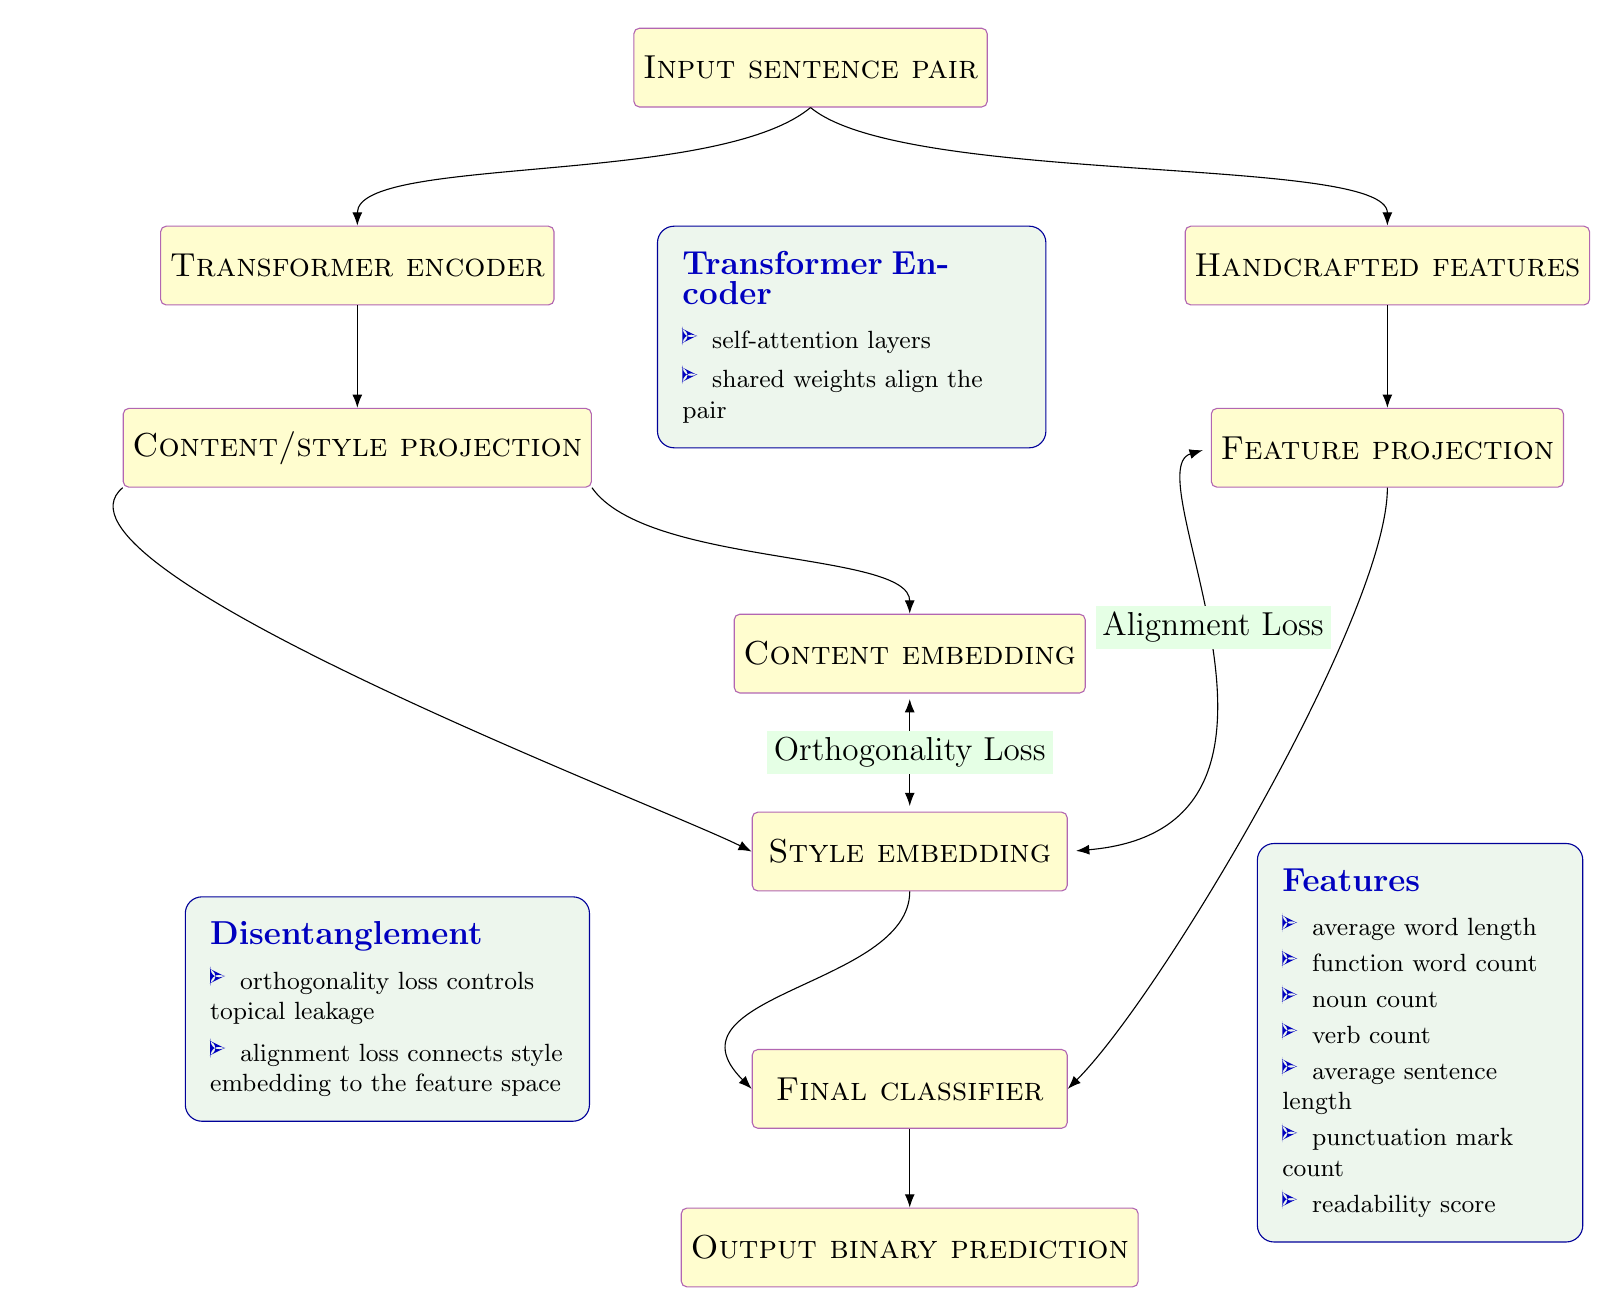
\begin{tikzpicture}

\node[box] (input) {\textsc{Input sentence pair}};

\node[box, below left = 1.5cm and 1cm of input] (trans)
      {\textsc{Transformer encoder}};
\node[box, below = 1.3cm of trans] (proj)
      {\textsc{Content/style projection}};

\node[box, below right = 1.6cm and 1.8cm of proj] (cont)
      {\textsc{Content embedding}};
\node[box, below = 1.5cm of cont] (style)
      {\textsc{Style embedding}};

\node[box, below right = 1.5cm and 2.5cm of input] (hand)
      {\textsc{Handcrafted features}};
\node[box, below = 1.3cm of hand] (feat)
      {\textsc{Feature projection}};

\node[box, below = 2.0cm of style] (final)
      {\textsc{Final classifier}};
\node[box, below = 1cm of final]   (out)
      {\textsc{Output binary prediction}};

\draw[->] (input.south)  .. controls +(-1.2,-1) and +(0,0.9) .. (trans.north);
\draw[->] (input.south)  .. controls +( 1.2,-1) and +(0,0.9) .. (hand.north);

\draw[->] (trans) -- (proj);
\draw[->] (proj.south east)
  .. controls +(0.7,-1) and +(0,0.8) .. (cont.north);

\draw[<->, shorten >=2pt, shorten <=2pt]
  (cont) -- (style) node[midway,loss]{Orthogonality Loss};

\draw[->] (proj.south west)
  .. controls +(-1.2,-1) and +(-1.2,0.6) .. (style.west);
\draw[->] (style.south)
  .. controls +(0,-1.2) and +(-1.2,1.2) .. (final.west);

\draw[->] (hand) -- (feat);

\draw[<->, shorten >=3pt, shorten <=3pt]
  (style.east) .. controls +(3.5,0.3) and +(-1,-0.3) .. (feat.west)
  node[midway,loss,above]{Alignment Loss};

\draw[->] (feat.south)
  .. controls +(0,-1.6) and +(1.2,1.2) .. (final.east);

\draw[->] (final) -- (out);


\node[
  exp,
  text width = 3.5cm,
  right  = 1.5cm of out.east,
  yshift = 2.6cm,
  anchor = west
] (feats)
{
  \textbf{\large\textcolor{blue!75!black}{Features}}\\[5pt]
  \bluebullet\; average word length\\[2pt]
  \bluebullet\; function word count\\[2pt]
  \bluebullet\; noun count\\[2pt]
  \bluebullet\; verb count\\[2pt]
  \bluebullet\; average sentence length\\[2pt]
  \bluebullet\; punctuation mark count\\[2pt]
  \bluebullet\; readability score
};

\node[exp,
      below left = 1.5cm and -0.3cm of input,
      anchor=north west, text width = 4.3cm] (encnote)
{
  \textbf{\large\textcolor{blue!75!black}{Transformer Encoder}}\\[5pt]
  \bluebullet\; self-attention layers\\[3pt]
  \bluebullet\; shared weights align the pair
};


\node[exp,
      text width = 4.5cm,      
      left   = 7.3cm of style.west,
      xshift = 0.1cm,
      yshift = -2.0cm,
      anchor = west] (explain)
{
  \textbf{\large\textcolor{blue!75!black}{Disentanglement}}\\[5pt]
  \bluebullet\; orthogonality loss controls\\topical leakage\\[4pt]
  \bluebullet\; alignment loss connects style\\embedding to the feature space
};

\end{tikzpicture}
\end{document}